\documentclass[a4paper,11pt]{article}

% --------------------------------------------------
%  Standard packages (unchanged)
% --------------------------------------------------
\usepackage[utf8]{inputenc}
\usepackage[T1]{fontenc}
\usepackage[english]{babel}
\usepackage{microtype}
\usepackage{csquotes}   
\usepackage{geometry}
\geometry{margin=2.5cm}
\usepackage{graphicx}
\usepackage{subcaption}
\usepackage{booktabs}
\usepackage{amsmath,amssymb}
\usepackage{siunitx}
\usepackage{hyperref}
\usepackage{cleveref}
\usepackage[
  backend=biber,
  style=authoryear,
  giveninits = true,
  uniquename = init,
  natbib
]{biblatex}
\addbibresource{../references.bib}

\begin{document}

\title{Analysis of Style Representation through Gram Matrices}
\author{Antonello Di Rita \\ Bachelor of Science in Artificial Intelligence}
\date{\today}
\maketitle

\begin{abstract}
\textbf{Aim} — To determine whether Gram matrices of convolutional feature activations encode \emph{art-historical style} well enough to distinguish movements such as \emph{Impressionism} or \emph{Baroque}.\\[2pt]
\textbf{Method} — Gram matrices are computed from five VGG-19 layers for paintings in the WikiArt dataset.  Pairwise root-mean-square error (RMSE) between matrices is analysed both \emph{before} and \emph{after} an explicit \emph{HSV-space normalisation} that rescales the saturation (\(S\)) and value (\(V\)) channels to zero mean and unit variance.\\[2pt]
\textbf{Results} — On raw images the Gram distances are dominated by global luminance and saturation, yielding almost no separation between conventional styles. After HSV normalisation, the gap between intra- and inter-style RMSE widens modestly - especially at the shallow \texttt{conv1\_1} layer—yet large overlaps remain.\\[2pt]
\textbf{Implications} — Gram matrices alone are a weak descriptor for canonical style classification.  Photometric preprocessing in HSV space is a \emph{necessary but insufficient} step toward exploiting these features in automatic style recognition.
\end{abstract}

\tableofcontents
\newpage

\section{Introduction}
The idea of encoding an image’s \emph{style} through \emph{Gram matrices} was introduced by \textcite{gatys2016} in their seminal work on \emph{image style transfer using convolutional neural networks}.
Given a pre-trained convolutional network such as VGG-19, each layer produces a set of feature maps that capture increasingly abstract representations of the input.  
Let $N_{l}$ be the number of filters in layer~$l$ and let $M_{l}$ be the total number of spatial positions in each feature map, i.e.\ the product of its height~$H_{l}$ and width~$W_{l}$.  
Thus the responses in layer~$l$ can be stored in a matrix $\boldsymbol{F}^{l}\in\mathbb{R}^{N_{l}\times M_{l}},$
where $\boldsymbol{F}^{l}_{ij}$ is the \emph{activation}—that is, the scalar output value (feature-map response) produced by the $i^{\text{th}}$ filter at spatial position~$j$—in layer~$l$.  
The Gram matrix is defined as
\begin{equation}
    G_{ij}^l = \sum_{k=1}^{M_l} F_{ik}^l \, F_{jk}^l,
    \label{eq:gram}
\end{equation}
namely the inner product between filters~$i$ and~$j$ at layer~$l$. In \textcite{gatys2016}, style transfer is achieved by back‑propagating a loss that matches the Gram matrices of a noise image to those of a reference artwork, while a second loss preserves the content of a separate content image.

\medskip
This study investigates \textbf{whether Gram matrices genuinely capture artistic style in the conventional art-historical sense}—for example \emph{Impressionism}, \emph{Baroque}, or \emph{Realism}.
A balanced subset of paintings was downloaded from the public \emph{WikiArt} repository via the \texttt{huggan/wikiart} dataset on Hugging Face.\footnote{\url{https://www.wikiart.org/}}
Style labels were provided by WikiArt.
Gram matrices were extracted from five layers of VGG-19 for each image, and pairwise similarity was measured using the RMSE between matrices.
Distance distributions for \emph{intra-style} and \emph{inter-style} pairs were compared to assess the discriminative power of the representation.
The entire procedure was repeated on images normalised for luminance and saturation to isolate purely chromatic effects.

\section{Dataset}
\subsection{Source: the \texttt{huggan/wikiart} corpus}
The original \textbf{WikiArt} collection on Hugging~Face\footnote{Dataset card: \url{https://huggingface.co/datasets/huggan/wikiart}} contains \num{81444} digitised
paintings by \num{129} artists annotated with \num{27} art‑historical styles, \num{11} genres,
and \num{129} artist identities. When downloaded as JPEG files, the archive occupies roughly \SI{70}{GB}.
Because the goal is to investigate the discriminative power of Gram matrices rather than to train a classifier,
a deliberately smaller subset is used.

\subsection{Subset construction}
A total of \textbf{100} images were randomly sampled. The sample spans \num{21} WikiArt styles; the four most
frequent—\textbf{Baroque}, \textbf{Impressionism}, \textbf{Realism}, and \textbf{Romanticism}—were retained
and each down‑sampled to six images to obtain a perfectly balanced working set of \num{24} paintings.

\subsection{Visual overview of the subset}
Figure~\ref{fig:samples} displays one representative thumbnail for each of the four selected styles.

\begin{figure}[htbp]
    \centering
    \begin{subfigure}[t]{.24\textwidth}
        \includegraphics[width=\linewidth]{../figures/Baroque.png}
        \caption{Baroque}
    \end{subfigure}
    \begin{subfigure}[t]{.24\textwidth}
        \includegraphics[width=\linewidth]{../figures/Impressionism.png}
        \caption{Impressionism}
    \end{subfigure}
    \begin{subfigure}[t]{.24\textwidth}
        \includegraphics[width=\linewidth]{../figures/Realism.png}
        \caption{Realism}
    \end{subfigure}
    \begin{subfigure}[t]{.24\textwidth}
        \includegraphics[width=\linewidth]{../figures/Romanticism.png}
        \caption{Romanticism}
    \end{subfigure}
    \caption{Representative paintings for the four art styles retained in the study.}
    \label{fig:samples}
\end{figure}

\section{Methodology}

\subsection{Network backbone}
The \textbf{VGG‑19} architecture introduced by \textcite{simon2014vgg} is adopted. Following \textcite{gatys2016}, every max‑pooling layer is replaced with an average‑pooling layer, exactly as done in the public implementation of \emph{Image Style Transfer Using Convolutional Neural Networks}\footnote{GitHub repository: \url{https://github.com/leongatys/PytorchNeuralStyleTransfer}}. This substitution improves the visual quality of the synthesised images used in neural style‑transfer and is retained here for consistency with that work.

\subsection{Feature layers and Gram extraction}
Each input painting is forward‑passed through VGG‑19, and the activations of the same five convolutional blocks used by \textcite{gatys2016} to define the style representation are recorded:
\begin{equation*}
    \{\text{conv1\_1},\;\text{conv2\_1},\;\text{conv3\_1},\;\text{conv4\_1},\;\text{conv5\_1}\}.
\end{equation*}
At each of these layers, a Gram matrix $G^{l}\in\mathbb{R}^{N_{l}\times N_{l}}$ is computed as in Equation~(\ref{eq:gram}).

\begin{figure}[htbp]
    \centering
    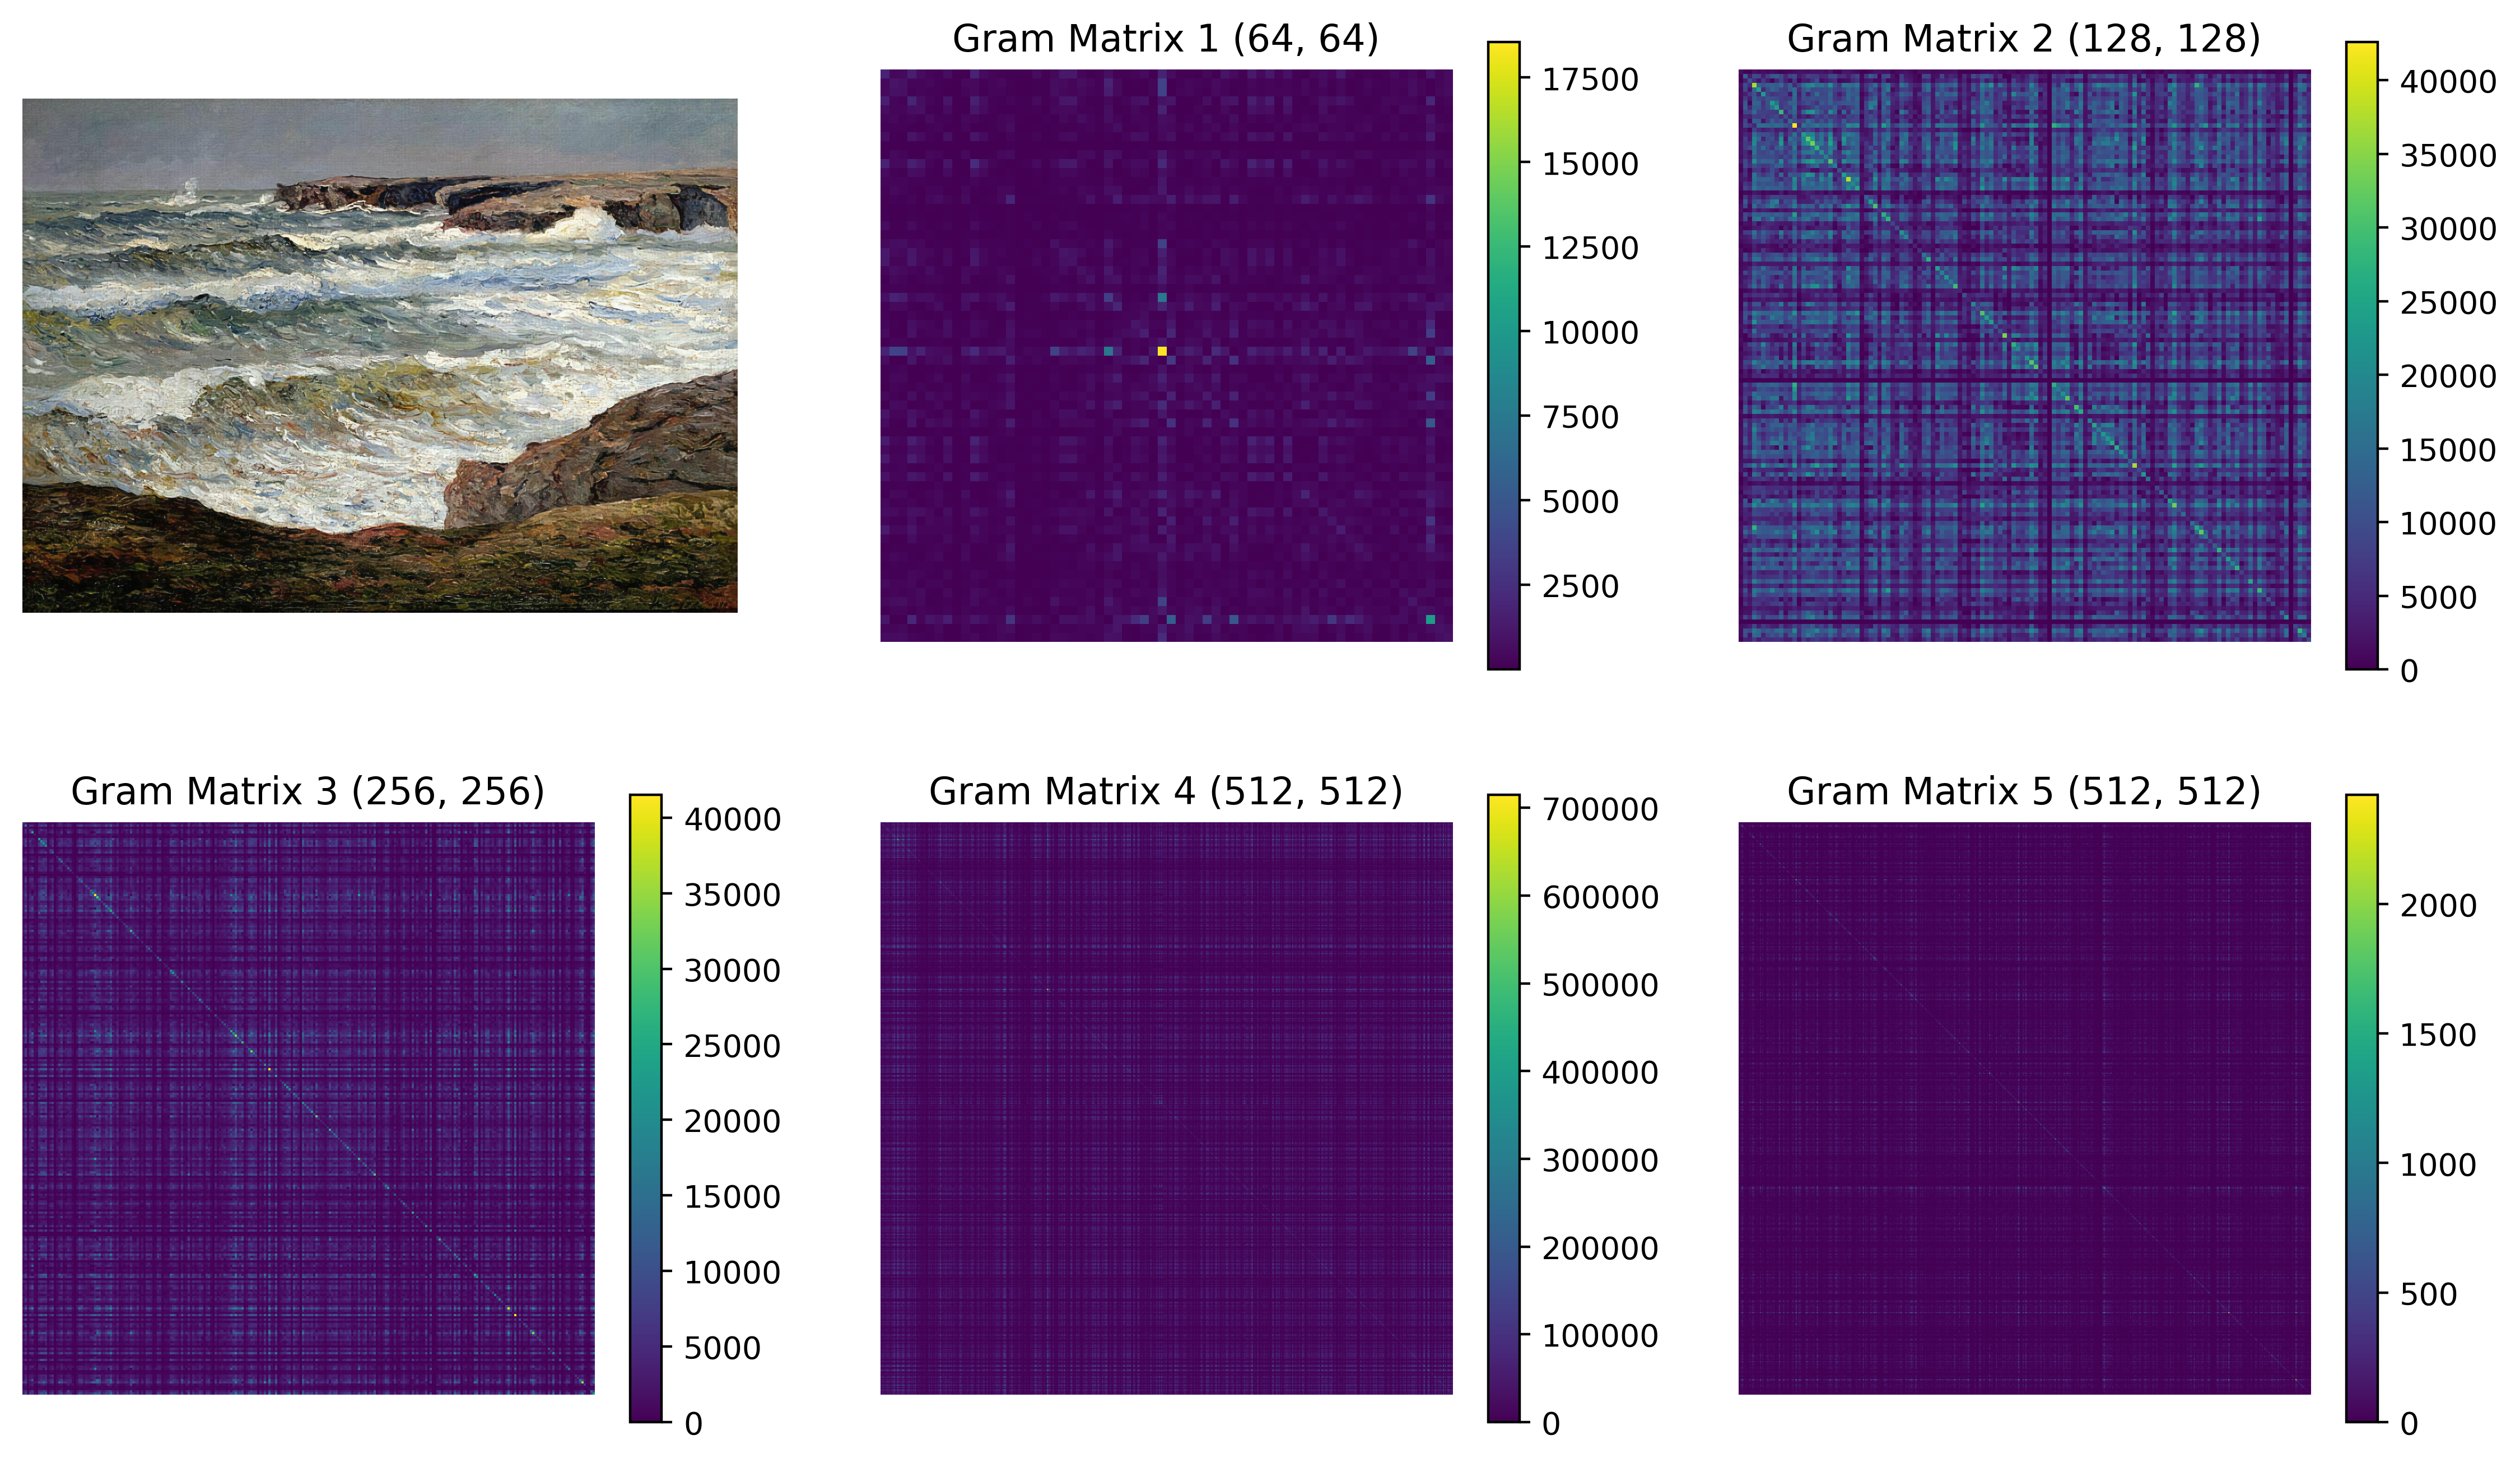
\includegraphics[width=0.8\linewidth]{../figures/Gram.png}
    \caption{Illustrative Gram matrices computed for one painting at the five VGG-19 layers (\texttt{conv1\_1}–\texttt{conv5\_1}) considered in this study. Brighter pixels denote higher filter-correlation values.}
    \label{fig:gram_example}
\end{figure}

\subsection{Pairwise similarity metric}
Given two Gram matrices $G^{l}_{A}$ and $G^{l}_{B}$ of the same dimensionality, their divergence is quantified using the root-mean-square error
\begin{equation}
    \operatorname{RMSE}(G^{l}_{A},G^{l}_{B}) = \sqrt{ \frac{1}{N_{l}^{2}} \sum_{i,j} \bigl(G^{l}_{A}(i,j)-G^{l}_{B}(i,j)\bigr)^{2} }.
\end{equation}

\subsection{Intra-style experiment}
Each of the four styles includes six paintings. All $\binom{6}{2}=15$ unordered pairs are evaluated, resulting in a $6\times6$ distance matrix with a zero diagonal. Figure~\ref{fig:rmse_intra} shows the intra-style distance matrices for the Impressionist subset at the five convolutional layers (\texttt{conv1\_1}–\texttt{conv5\_1}). Each matrix reports the RMSE between Gram matrices of image pairs.

\begin{figure}[ht]
  \centering
  \includegraphics[width=\textwidth]{../figures/Impressionism_RMSE.png}
  \caption{Intra-style distance matrices for the Impressionist subset at convolutional layers \texttt{conv1\_1}, \texttt{conv2\_1}, \texttt{conv3\_1}, \texttt{conv4\_1} and \texttt{conv5\_1}. Each panel is a $6\times6$ matrix where the entry at position $(i,j)$ represents the RMSE between the Gram matrices of image~$i$ and image~$j$. The diagonal is zero by definition. Images are indexed consistently across the matrix and are shown on the left in a $3\times2$ grid; the $i$-th row and column correspond to the $i$-th image in this grid.}
  \label{fig:rmse_intra}
\end{figure}

\subsection{Inter-style experiment}
Then, images from each pair of different movements are compared. Given styles \(s_{a}\) and \(s_{b}\) (each with six images), a \(12\times12\) block matrix is formed whose top-left and bottom-right quadrants correspond to the intra-style distances already analysed, while the off-diagonal blocks capture the \emph{inter-style} distances. Figure~\ref{fig:rmse_inter} shows these inter-style distance matrices for the Baroque vs.\ Impressionism pair at the five convolutional layers (\texttt{conv1\_1}–\texttt{conv5\_1}). The working hypothesis is that the intra-style quadrants (I and IV) exhibit lower RMSE than the inter-style quadrants (II and III).

\begin{figure}[ht]
  \centering
  \includegraphics[width=\textwidth]{../figures/Baroque_Impressionism_RMSE.png}
  \caption{Inter-style distance matrices for the Baroque vs.\ Impressionism pair at convolutional layers \texttt{conv1\_1}, \texttt{conv2\_1}, \texttt{conv3\_1}, \texttt{conv4\_1} and \texttt{conv5\_1}. Each panel is a \(12\times12\) block matrix: quadrants~I and~IV show intra-style distances (with zeros on the diagonal), while quadrants~II and~III contain inter-style distances. The 12 images (6 per style) are ordered consistently across rows and columns and are displayed on the left in a $4\times3$ grid; the $i$-th row and column correspond to the $i$-th image in this grid.}
  \label{fig:rmse_inter}
\end{figure}

\subsection{Aggregated statistics and visualisation}
For each convolutional layer, the following metrics are computed:
\begin{itemize}
    \item the mean intra‐style RMSE for each style \(s\), averaged over its \(\binom{6}{2}=15\) same‐style image pairs;
    \item the mean inter‐style RMSE for each unordered style pair \((s_a,s_b)\), averaged over all \(6\times6=36\) cross‐style image pairs.
\end{itemize}
These per‐layer values are plotted as grouped bars in Figure~\ref{fig:rmse_barplot}: one bar for each of the four styles (intra) and one bar for each of the six style combinations (inter).

\begin{figure}[htbp]
    \centering
    \includegraphics[width=\textwidth]{../figures/barplot_RMSE.png}
    \caption{Per‐layer grouped bar plot of average intra‐style RMSE (one bar per style) and average inter‐style RMSE (one bar per style pair). Lower values indicate greater similarity.}
    \label{fig:rmse_barplot}
\end{figure}

\subsection{Mitigating colour and brightness bias}\label{sec:norm_experiments}
The similarity scores reported so far may be confounded by global differences in luminance and saturation.  
To address this, two complementary normalisation schemes are explored, applied prior to computing the Gram matrices.

\subsubsection{Feature-space normalisation}
At each convolutional layer, the channel-wise mean is subtracted and the result divided by the channel-wise standard deviation, computed independently for every filter and every input image:
\begin{equation}
  \tilde{\mathbf{F}}_{i}=\frac{\mathbf{F}_{i}-\boldsymbol{\mu}_{i}}{\boldsymbol{\sigma}_{i}},
  \qquad
  \boldsymbol{\mu}_{i}=\textstyle\frac{1}{HW}\sum_{h,w}\mathbf{F}_{i}(h,w),
  \qquad
  \boldsymbol{\sigma}_{i}=\sqrt{\frac{1}{HW}\sum_{h,w}\bigl(\mathbf{F}_{i}(h,w)-\boldsymbol{\mu}_{i}\bigr)^{2}+\varepsilon},
  \label{eq:featnorm}
\end{equation}
where \(H\) and \(W\) are the spatial dimensions and \(\varepsilon\) ensures numerical stability.
\footnote{Implementation note (PyTorch):
\texttt{Z = (X - X.mean(dim=(2,3), keepdim=True)) / (X.std(dim=(2,3), unbiased=True, keepdim=True) + $\varepsilon$)}.}
Gram matrices are then recomputed from the normalised activations. Figure~\ref{fig:gram_norm} shows the resulting inter-style Gram matrices after normalisation.

\begin{figure}[htbp]
  \centering
  \includegraphics[width=\textwidth]{../figures/rmse_featurenorm.png}
  \caption{Example inter-style Gram matrices after \emph{feature-space} normalisation.}
  \label{fig:gram_norm}
\end{figure}

\subsubsection{Image-space normalisation in HSV}
The second normalisation scheme operates directly on the input images. Each RGB image is first converted to the HSV colour space, where the \emph{H} channel encodes hue, \emph{S} saturation, and \emph{V} value (brightness).The \(S\) and \(V\) channels are then rescaled to have zero mean and unit variance over the entire image—leaving the \(H\) channel unchanged—and the result is converted back to RGB before being fed into VGG.

\begin{figure}[htbp]
  \centering
  \includegraphics[width=\textwidth]{../figures/HSV_normalized.png}
  \caption{Thumbnails of images after \emph{HSV} normalisation.}
  \label{fig:hsv_examples}
\end{figure}

\subsection{Updated similarity metrics (HSV only)}\label{sec:updated_metrics}
All RMSE scores are recomputed using the HSV-normalised inputs.
Figure~\ref{fig:rmse_inter_norm} reports the inter-style distance matrices for Baroque versus Impressionism (cf.\ Fig.~\ref{fig:rmse_inter}), while Fig.~\ref{fig:rmse_barplot_norm} updates the grouped bar plot of intra- and inter-style means.

\begin{figure}[htbp]
  \centering
  \includegraphics[width=\textwidth]{../figures/rmse_norm_inter.png}
  \caption{Inter-style RMSE (Baroque vs.\ Impressionism) computed from \emph{HSV-normalised} images.}
  \label{fig:rmse_inter_norm}
\end{figure}

\begin{figure}[htbp]
  \centering
  \includegraphics[width=\textwidth]{../figures/rmse_barplot_norm.png}
  \caption{Grouped bar plot of average intra-style (one bar per style) and inter-style (one bar per style pair) RMSE, based on \emph{HSV-normalised} inputs.}
  \label{fig:rmse_barplot_norm}
\end{figure}

\section{Results and Discussion}

The analysis conducted clearly highlights how \emph{Gram matrices} are strongly dependent on the specific characteristics of the analysed images rather than on a stable, generalised representation of artistic style. In particular, saturation and luminance exert a significant influence on the Gram matrices. This result was partially expected, since the original neural style‑transfer paper transfers saturation and luminance properties as well. Less anticipated was the magnitude of this effect: it is so strong that pairs of images belonging to different artistic movements often exhibit lower RMSE than pairs of images from the same movement but with different luminance or saturation.

Hence, using Gram matrices for reliable classification of artistic style—understood as conventional art movements—proves problematic because of this intrinsic variability.

In the second part of the study, standardising the feature activations did not significantly reduce this variability or improve style classification. By contrast, pre‑standardising the images in the HSV colour space confirmed the hypothesis that luminance and saturation strongly influence the Gram matrices. After this normalisation a clear trend emerges: intra‑style pairs show, on average, lower RMSE than inter‑style pairs, although numerous exceptions remain that still prevent this representation from being used for robust classification.

Interestingly, after HSV normalisation the gap between intra‑ and inter‑style RMSE is \textbf{most pronounced} when the Gram matrices are computed from the activations of the \texttt{conv1\_1} layer. This observation suggests that the style cues most consistent with traditional art‑historical movements may already be encoded at this shallow level of the network, where low‑level features—such as brush‑stroke texture and coarse colour patterns—are represented. Providing a precise semantic interpretation of these early‑layer correlations, however, remains an open challenge.

Several considerations arise:
\begin{itemize}
\item The images extracted from the dataset may not effectively represent the associated art movement, negatively affecting the coherence of the results.
\item Rows or columns with significantly higher RMSE associated with single images might indicate an overly inclusive labelling in the original dataset; images showing only a hint of Impressionism, for instance, may have been categorised outright as Impressionist.
\item A stricter selection criterion based on RMSE values could enable more coherent subsets of images that are genuinely representative of the analysed styles.
\item The information captured by Gram matrices may be quite specific rather than broad. The variability within each art movement could be too great to be effectively represented by Gram matrices.
\item Grouping images by the personal style of individual artists (e.g., Van Gogh or Monet) rather than by broad movements might be more effective, as it could capture recurring, distinctive characteristics within an artist’s oeuvre, considerably lowering intra‑group RMSE and improving discrimination.
\end{itemize}

\printbibliography

\end{document}
